\documentclass[12pt]{article}
\usepackage[dvips,xetex]{graphicx}
\usepackage{ifpdf}
\usepackage{amsmath,amsthm,amsfonts}
\usepackage{unicode-math}
\usepackage[margin=1.0in]{geometry}
\usepackage{subfigure}
\usepackage{changepage}
\usepackage{ragged2e}
\usepackage[export]{adjustbox}
\usepackage{hanging}
\usepackage[all]{nowidow}
\usepackage{float}
\usepackage[font=footnotesize]{caption}
\captionsetup[figure]{labelformat=empty}
\pagenumbering{gobble}

\begin{document}

\begin{flushleft}
   \begin{footnotesize}
      Corresponding author:
      Mary Forrester\\
Colorado School of Mines\\
mforrest@mymail.mines.edu
   \end{footnotesize}
\end{flushleft}

\begin{center}
   \textbf{The day that Cupcake took over the world}
\end{center}

\begin{center}
   \begin{footnotesize}
      Joseph O'Neill, Appalachian State University\\
Mary Forrester, Colorado School of Mines\\
Cupcake the Terror, the Organization for Neurotic Pups\\
Michael Morse, Integrated GroundWater Modeling Center\\
Your Mom
   \end{footnotesize}
\end{center}

\begin{adjustwidth}{0.5in}{0.5in}
\begin{footnotesize}
   \setlength{\parindent}{0cm}
   \textbf{Abstract:} Here is an abstract copied from MM Proceedings, 2015. Groundwater from the Chalk aquifer beneath London is an important resource for the city's water supply
and has a long and complex history of development. Intense abstraction in the period 1920 to 1960
(approximately 450,000 m3
/day) led to extensive drawdown but subsequently abstraction rates have
decreased and groundwater levels have been rising, leading to the potential for re-saturation of the
confining clays. This has required a detailed monitoring programme and adjustments to the abstraction
regime to stabilise groundwater at levels such that there is no threat to the stability of infrastructure whilst
providing sufficient water resources and protecting the needs of the environment. 
\end{footnotesize}
\end{adjustwidth}
\vspace{3mm}

\begin{flushleft}
\textbf{Extended abstract: Methodology, findings, and implications}
\end{flushleft}
Here is some text copied from MM Proceedings 2015. The London Basin is a broadly easterly-plunging synclinal structure between the Chiltern Hills to the north and the North Downs in the south. The main aquifer unit comprises Chalk with a layer of fine sand at the top (the Thanet Sands), and is confined across much of the city by up to 80 m of clayey Tertiary deposits
(principally the London Clay and Lambeth Group). A simplified geological map is shown in Figure 1.

Recharge to the aquifer occurs where the Chalk is at outcrop and unconfined to the north and south of the city of London. Groundwater from the Chalk aquifer beneath London is an important resource for the city's water supply and has a long and complex history of development.Before the 1800s London's water supply came from the River Thames and its tributaries, and from shallow wells in near-surface gravel deposits. Through the 1800s there was growing concern that the shallow groundwater was, in some areas, not fit to drink. Meanwhile deep drilling techniques were improving, so the deeper, locally artesian Chalk aquifer was increasingly exploited. 

During the period 1920 to 1960net abstraction from the confined Chalkwas approximately 450,000 m3/day, approximately equal to modern estimates of the total groundwater flow into the confined aquifer (ESI, 2013). Historically the Chalk aquifer discharged at the eastern end of the Thames estuary, but this overabstraction caused considerable drawdown in the Chalk. Groundwater levels reached 90 m below sea level in the centre of the depression around Trafalgar Square (Figure 2), and the Chalk aquifer became unconfined beneath a large part of the city. Issues with saline intrusion were encountered along the northern bank of the Thames where the aquifer crops out beneath the estuary (Mott MacDonald, 2003). Groundwater abstraction rates dropped throughout the 1970s to the 1990s, leading to a sharp rebound in groundwater levels in the confined aquifer. Infrastructure developed since the Chalk aquifer became unconfined in the 1920s (including much of the London Underground system) was now thought to be at risk of ground movement due to re-saturation of the overlying clays. This has required a detailed monitoring programme and adjustments to the abstraction regime to stabilise groundwater at levels such that there is no threat to the stability of infrastructure whilst providing sufficient water resources (Environment Agency, 2014). Groundwater levels have been actively managed to mitigate this risk by the General Aquifer Research Development and Investigation Team (GARDIT), established in 1998. Artificial recharge schemes have also been developed to take advantage of the unconfined storage in parts of the aquifer. 

I would also like to demonstrate using math and other symbols within this form. I can insert unicode text directly into the document, as long as I use a dollar sign before an after the symbols. For instance, $∫₀³ xⁿφ₁₂(x)$. Using the double dollar signs centers the formula and begins a new line:
$$ ∫₀³ xⁿφ₁₂(x) $$
The form also allows many basic LaTeX commands:
$$
F(s)=\mathscr L \{f(t)\}=\int_0^\infty \mathrm e^{-st}f(t)\,\mathrm d t 
$$

Ok, after the math demonstration let's just add some more text to show a bit more formatting. The max characters allowed for this field is 7000. Ok, after the math demonstration let's just add some more text to show a bit more formatting. The max characters allowed for this field is 7000. Ok, after the math demonstration let's just add some more text to show a bit more formatting. The max characters allowed for this field is 7000. Ok, after the math demonstration let's just add some more text to show a bit more formatting. The max characters allowed for this field is 7000. Ok, after the math demonstration let's just add some more text to show a bit more formatting. The max characters allowed for this field is 7000. Ok, after the math demonstration let's just add some more text to show a bit more formatting. The max characters allowed for this field is 7000. Ok, after the math demonstration let's just add some more text to show a bit more formatting. The max characters allowed for this field is 7000. Ok, after the math demonstration let's just add some more text to show a bit more formatting. The max characters allowed for this field is 7000. Ok, after the math demonstration let's just add some more text to show a bit more formatting. The max characters allowed for this field is 7000. Ok, after the math demonstration let's just add some more text to show a bit more formatting. The max characters allowed for this field is 7000. Ok, after the math demonstration let's just add some more text to show a bit more formatting. The max characters allowed for this field is 7000. Ok, after the math demonstration let's just add some more text to show a bit more formatting. The max characters allowed for this field is 7000. 



\begin{figure}[H]
   \centering
   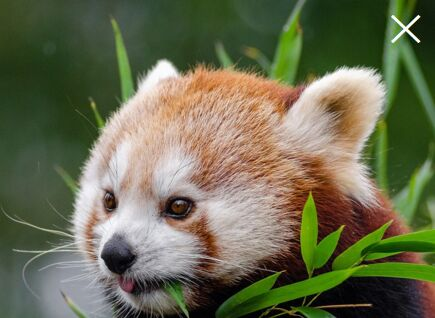
\includegraphics[max width=\textwidth]{redpanda.jpg}
   \caption{Figure 1: SO CUTE. Let's go to the zoo! I can add up to two images of file types pdf, jpg, or png. The uploaded file must not exceed 5 MB. If the width of the image exceeds the text width of the document, the image is automatically resized to 5 inches. User must label their figure or table caption with "Figure 1:...". Also, there is an unfortunate bug where the form stops auto-saving as soon as you upload an image. Hoping to fix that...}
\end{figure}

\begin{figure}[H]
   \centering
   
\includegraphics[max width=\textwidth]{Default.png}
   \caption{ }
\end{figure}

\begin{center}
   \textbf{References}
\end{center}
\begin{footnotesize}
   \setlength{\parindent}{0cm}
   \setlength{\parskip}{0.25cm}
   Hey. Here are some example references copied from the MODFLOW and More Proceedings, 2015.

Crossrail Ltd, 2010. Groundwater level monitoring. Document Number: CRL1-GCG-C2-RAN-CRG03-
00002.

Environment Agency, 2002.Enhancements to Modflow.Variations in hydraulic conductivity and storage
with depth. National Groundwater and Contaminated Land Centre project NC/00/23.

Environment Agency, 2014.Management of the London Basin Chalk Aquifer Annual Status Report
2014. https://www.gov.uk/government/publications/london-basin-chalk-aquifer-annual-status-report

ESI, 2013. London Basin Aquifer: Numerical Model Report. Report reference: 60121 R2. ESI Limited,
Shrewsbury, UK.

FAO, 1998.Crop evapotranspiration, Guidelines for computing crop water requirements.FAO Irrigation and

Drainage Paper 56.Food and Agriculture Organisation of the United Nations, Rome.

Harbaugh, A.W. and McDonald, M.G., 1988. A modular three-dimensional finite-difference groundwater
flow model.US Geological Survey.Scientific software group, Washington DC.

Heathcote, J.A., Lewis, R.T. and Soley, R.W.N. 2004. Rainfall routing to runoff and recharge for regional
groundwater resource models. Quarterly Journal of Engineering Geology and Hydrogeology, 37,
113-130.

Mott MacDonald, 2003. LBGM Report on Model Upgrade and Re-Calibration. 61993EA01. Mott
MacDonald, Cambridge, UK.

Prudic, D.E., 1989. Documentation of a computer program to simulatestream-aquifer relations using a
modular, finite-difference, ground-waterflow model: U.S. Geological Survey Open-File Report 88-
729, 113 p.

Simpson, B., Blower, T., Craig, R.N., Wilkinson, W.B., 1989.The engineering implications of rising
groundwater levels in the deep aquifer beneath London.CIRIA Special Publication 69. 
\end{footnotesize}

\end{document}
